% CMAI 2026 - `python talk/slides.py --beamer` ilə qurulub. ƏL İLƏ REDAKTƏ ETMƏ:
% məzmun `talk/slides.py` faylındadır, bu fayl hər qurulmada üstündən yazılır.
%
% XELATEX İLƏ KOMPİLYASİYA ET, pdflatex ilə YOX:
%     xelatex slides.tex
% Səbəb: nümunələrdə `ə` (U+0259) var və standart pdflatex şriftlərində yoxdur.
\documentclass[aspectratio=169,12pt]{beamer}
\usetheme{default}
\usepackage{fontspec}
\usepackage{booktabs}
\usepackage{graphicx}
\usepackage{xcolor}
\setmainfont{Segoe UI}
\setsansfont{Segoe UI}

% Rənglər `talk/figures.py`-dakı təsdiqlənmiş palitra ilə eynidir, yəni
% slaydla qrafik proyektorda eyni mavini göstərir.
\definecolor{accent}{HTML}{2a78d6}
\definecolor{ink}{HTML}{0b0b0b}
\definecolor{inksoft}{HTML}{52514e}
\definecolor{muted}{HTML}{898781}
\definecolor{surface}{HTML}{fcfcfb}

% Fon PPTX versiyası ilə eyni isti ağdır, xalis ağ deyil.
\setbeamercolor{background canvas}{bg=surface}

\setbeamercolor{frametitle}{fg=ink,bg=}
\setbeamercolor{title}{fg=ink}
\setbeamercolor{author}{fg=inksoft}
\setbeamercolor{institute}{fg=inksoft}
\setbeamercolor{date}{fg=inksoft}
\setbeamercolor{normal text}{fg=ink}
\setbeamerfont{frametitle}{size=\large,series=\bfseries}

% Başlığın altında vurğu zolağı, PPTX versiyası ilə eyni.
\setbeamertemplate{frametitle}{%
  \vspace{0.45cm}%
  \usebeamerfont{frametitle}\usebeamercolor[fg]{frametitle}\insertframetitle\par
  \vspace{0.12cm}%
  \hspace*{0.02\textwidth}\textcolor{accent}{\rule{0.10\textwidth}{2.2pt}}%
}

\setbeamertemplate{navigation symbols}{}
\setbeamertemplate{footline}[frame number]
\setbeamercolor{footline}{fg=inksoft}

\title{AZ-Eval: A Parallel Azerbaijani–English Benchmark Reveals Negative Cross-Lingual Transfer from Kazakh Fine-Tuning}
\author{Nihat Garibli}
\institute{Baku State University, Azerbaijan}
\date{CMAI 2026 · Nazarbayev University, Astana}

\begin{document}

% Başlıq səhifəsi əl ilə qurulur. Beamer-in `\titlepage` komandası mətni
% mərkəzə yığır və PPTX versiyası ilə uyuşmur; sola düzləndirmə və vurğu
% zolağı iki formatı eyni görkəmə gətirir.
\begin{frame}[plain]
  \vspace{1.4cm}
  \hspace*{0.02\textwidth}\textcolor{accent}{\rule{0.22\textwidth}{4pt}}\par
  \vspace{0.55cm}
  \hspace*{0.02\textwidth}\parbox{0.95\textwidth}{\raggedright
    {\LARGE\bfseries\color{ink} AZ-Eval: A Parallel Azerbaijani–English Benchmark Reveals Negative Cross-Lingual Transfer from Kazakh Fine-Tuning}\par
    \vspace{0.85cm}
    {\large\color{inksoft} Nihat Garibli}\par
    \vspace{0.12cm}
    {\color{inksoft} Baku State University, Azerbaijan}\par
    \vspace{1.1cm}
    {\small\color{muted} CMAI 2026 · Nazarbayev University, Astana}
  }
\end{frame}

\begin{frame}{Open multilingual models are measured on high-resource languages}
\begin{itemize}
  \item[] Kazakh has open evaluation sets - freshqa\_kazakh, defan\_kazakh, BeyneleBench
  \item[] Azerbaijani, to our knowledge, has none
\vspace{0.25cm}
  \item[] Both are Turkic. Kazakh is written in Cyrillic, Azerbaijani in Latin.
\end{itemize}
\note{One sentence only: this is the host institute's own methodology, extended to another Turkic language. Do not linger.}
\end{frame}

\begin{frame}{The question}
\begin{center}{\large\bfseries Does fine-tuning on Kazakh transfer to Azerbaijani?}\end{center}
\vspace{0.3cm}
\begin{itemize}
\vspace{0.25cm}
  \item[] Kazakh is the closest well-resourced Turkic relative of Azerbaijani.
  \item[] Adapting to a related language is the intuitive move for a low-resource language.
\end{itemize}
\note{Stress the script difference now. It detonates on slide 8.}
\end{frame}

\begin{frame}{AZ-Eval - an open parallel benchmark}
\begin{center}{\large\bfseries verified\_by is a gate, not metadata: unverified rows never enter the set.}\end{center}
\vspace{0.3cm}
\begin{center}
\begin{tabular}{lr}
\toprule
356 parallel AZ/EN short-answer items & 255 hand-written by a native speaker \\
Every item human-verified & 101 from templated Wikidata queries \\
7 categories & math, history, geography, science, culture, language, world \\
Accepted answers expanded & rule-based Azerbaijani morphology \\
\bottomrule
\end{tabular}
\end{center}
\vspace{0.3cm}
\note{Say in one sentence why the questions are not about Azerbaijan: we need facts the model demonstrably knows in English, otherwise the gap collapses to zero and measures nothing. Otherwise it comes back in Q\&A.}
\end{frame}

\begin{frame}{Four nested normalizations}
\begin{center}{\large\bfseries STRICT  →  MORPH  →  LENIENT  →  TRANSLIT}\end{center}
\vspace{0.3cm}
\begin{itemize}
\vspace{0.25cm}
  \item[] suffix stripping   ·   diacritic folding   ·   Cyrillic→Latin
\vspace{0.25cm}
  \item[] Each stage adds exactly one transformation, applied symmetrically to
  \item[] prediction and reference - so each score increment attributes error mass
  \item[] to that single surface phenomenon.
\vspace{0.25cm}
  \item[] Paired comparisons · 1000-resample bootstrap · permutation test · Holm correction
\end{itemize}
\note{This is a mathematics conference. Showing bare percentages looks weak; showing that the measurement is trustworthy looks strong. Do not claim a theorem.}
\end{frame}

\begin{frame}{Result 1 - the gap is universal}
\begin{center}{\large\bfseries Majority-class baseline: 1.1\%}\end{center}
\vspace{0.3cm}
\begin{center}
\begin{tabular}{lrrrr}
\toprule
\textbf{Model} & \textbf{AZ} & \textbf{EN} & \textbf{Gap} & \textbf{p (Holm)} \\
\midrule
Qwen3-1.7B & 5.9\% & 23.6\% & 17.7 & 0.0016 \\
Qwen3-VL-4B-Instruct & 16.6\% & 30.6\% & 14.0 & 0.0016 \\
issai/Qolda-AVL-5B & 3.1\% & 29.5\% & 26.4 & 0.0016 \\
\bottomrule
\end{tabular}
\end{center}
\vspace{0.3cm}
\note{'Every model is bad at Azerbaijani' is the expected result - do not dwell. Point at the last row and move on: something is wrong there.}
\end{frame}

\begin{frame}{Result 2: transfer is NEGATIVE}
\begin{center}

\includegraphics[width=0.80\textwidth]{fig_negative_transfer}
\end{center}
\vspace{-0.15cm}
\begin{center}{\small\color{inksoft} Holm-corrected p = 0.0024   ·   same architecture, same quantization, same prompt}\end{center}
\note{Stop here. This is the centre of the talk. Do not rush. The only difference between the two models is the Kazakh fine-tune.}
\end{frame}

\begin{frame}{The mechanism is orthographic}
\begin{center}
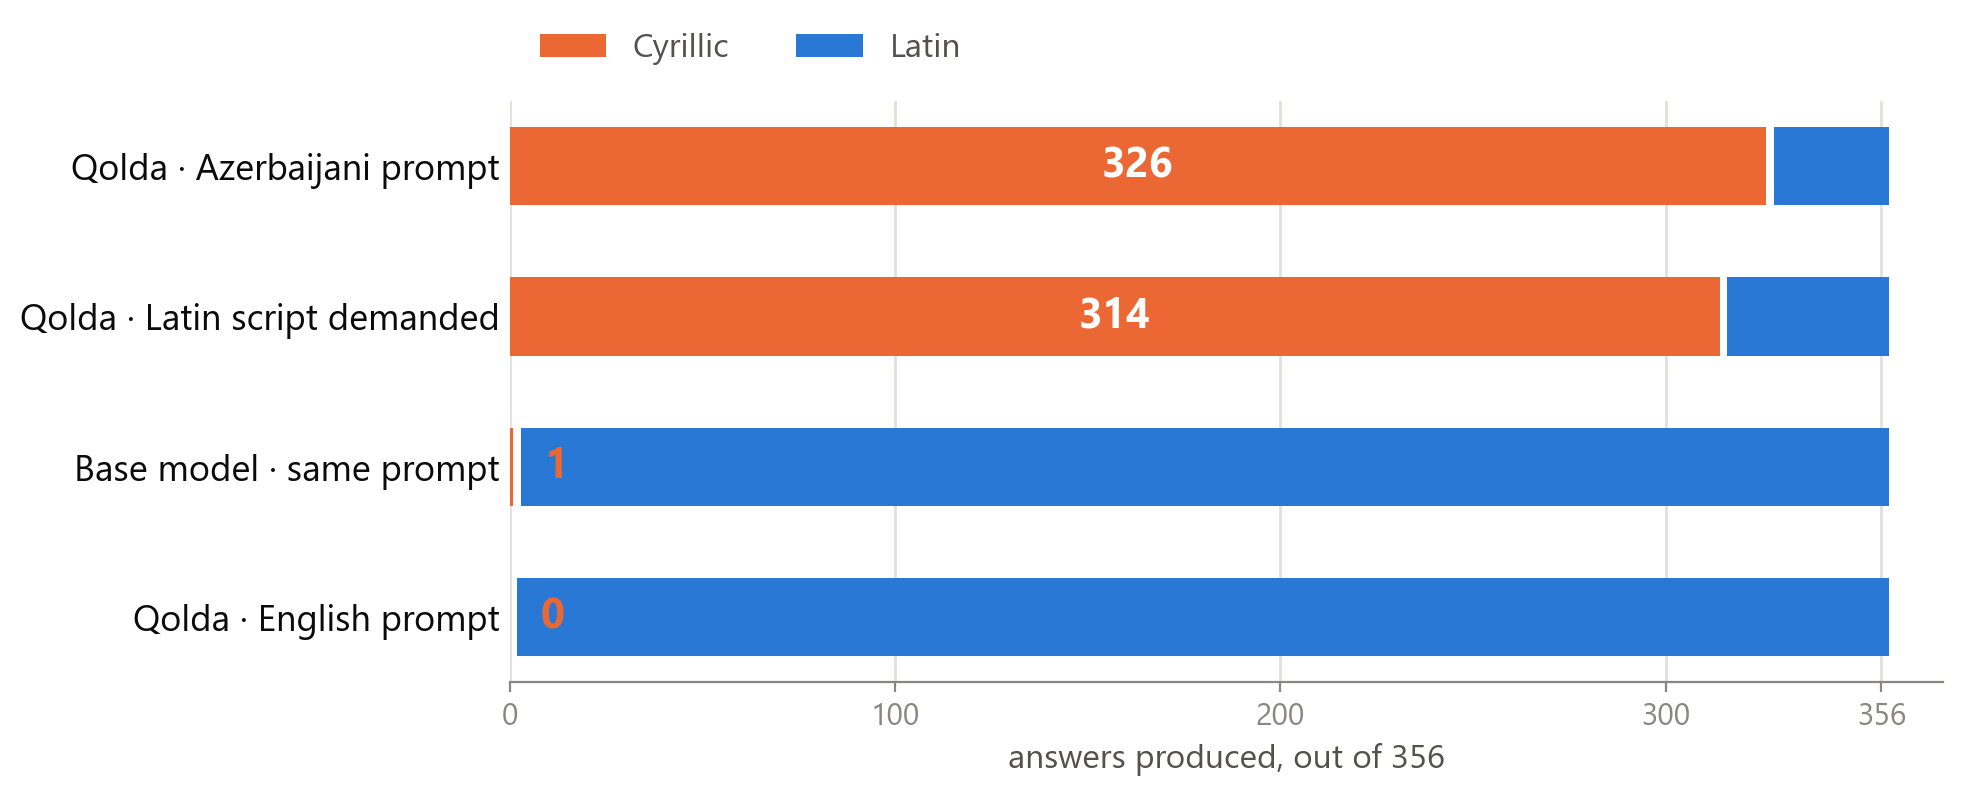
\includegraphics[width=0.80\textwidth]{fig_script_counts}
\end{center}
\vspace{-0.15cm}
\begin{center}{\small\color{inksoft} Understands the question, finds the answer, writes it in the wrong alphabet.}\end{center}
\note{The memorable moment of the talk. Slow down. Two sentences: 326 vs 1 is a direct count, it depends on no statistical test. And demanding the Latin alphabet in the prompt moves only 12 of the 326.}
\end{frame}

\begin{frame}{Is it simply a weaker model?}
\begin{center}{\large\bfseries Indistinguishable in English. 35.4 points apart in Azerbaijani.}\end{center}
\vspace{0.3cm}
\begin{center}
\begin{tabular}{lrrrr}
\toprule
\textbf{Language} & \textbf{Base model} & \textbf{Kazakh-tuned} & \textbf{Gap} & \textbf{p (Holm)} \\
\midrule
English & 59.4\% & 59.4\% & 0.0 & 1.0000 \\
Azerbaijani (STRICT) & 45.8\% & 10.4\% & 35.4 & 0.0030 \\
\bottomrule
\end{tabular}
\end{center}
\vspace{0.3cm}
\begin{itemize}
  \item[] 96 world + science items - facts every model demonstrably knows in English
\end{itemize}
\note{A weaker model would be weaker in both languages. This one is weaker only in Azerbaijani. Raise the objection before the audience does.}
\end{frame}

\begin{frame}{Takeaway}
\begin{center}{\large\bfseries Dataset CC BY 4.0 · Code MIT · github.com/nihatgaribli/AZ-Eval}\end{center}
\vspace{0.3cm}
\begin{itemize}
  \item[] 1.  Fine-tuning on a closely related language can HARM rather than help
  \item[]      - when the writing systems differ.
\vspace{0.25cm}
  \item[] 2.  Most of the damage is orthographic, not semantic
  \item[]      - transliteration removes 56\% of the deficit.
\vspace{0.25cm}
  \item[] 3.  Which means it is in principle fixable
  \item[]      - e.g. by constraining the output script at decoding time.
\end{itemize}
\note{End on the practical sentence. Someone building a low-resource model is in this room.}
\end{frame}

\appendix
\begin{frame}
  \begin{center}{\Large Backup slides}\end{center}
\end{frame}

\begin{frame}{Backup - where the gap is widest}
\begin{center}{\large\bfseries Mathematics: knowledge is present in English, the language blocks it.}\end{center}
\vspace{0.3cm}
\begin{center}
\begin{tabular}{lrrr}
\toprule
\textbf{Category} & \textbf{n} & \textbf{Qwen3-VL-4B (AZ / EN)} & \textbf{Qolda-AVL-5B (AZ / EN)} \\
\midrule
mathematics & 28 & 3.6\% / 25.0\% & 3.6\% / 28.6\% \\
world & 45 & 51.1\% / 57.8\% & 0.0\% / 60.0\% \\
history & 45 & 4.4\% / 0.0\% & 0.0\% / 2.2\% \\
\bottomrule
\end{tabular}
\end{center}
\vspace{0.3cm}
\note{Keep this ready - it is a mathematics conference and this is the widest gap. History sits near zero in BOTH languages: that is ignorance, not a script problem.}
\end{frame}

\begin{frame}{Backup - what survives transliteration}
\begin{itemize}
  \item[] Transliteration removes 56\% of the deficit - but not all of it.
\vspace{0.25cm}
  \item[] Residual after TRANSLIT: 5.9 points, Holm p = 0.0364 - still significant.
\vspace{0.25cm}
  \item[] So the claim is: the damage is LARGELY orthographic, not purely orthographic.
\end{itemize}
\note{Honest framing. At n=96 this residual was not detectable; at n=356 it is.}
\end{frame}

\begin{frame}{Backup - how the dataset was built}
\begin{itemize}
  \item[] 255 items hand-written by a native Azerbaijani speaker
  \item[] 101 from 8 templated SPARQL queries × 4 syntactic variants (round-robin)
\vspace{0.25cm}
  \item[] No LLM authored, translated, or answered any dataset item.
  \item[] Rejected candidates are retained, so the acceptance rate stays auditable.
\vspace{0.25cm}
  \item[] Items whose gold answer depends on a contested position are excluded (6 removed).
\end{itemize}
\end{frame}

\begin{frame}{Backup - limitations}
\begin{itemize}
  \item[] n = 356. Confidence intervals are ±2–5 points; every reported comparison
  \item[] survives Holm correction.
\vspace{0.25cm}
  \item[] One model pair. The 9B/8B pair did not fit in 8 GB of VRAM.
\vspace{0.25cm}
  \item[] Two knowledge regimes are mixed on purpose - and kept in separate categories
  \item[] so the distinction stays visible instead of averaging away.
\end{itemize}
\end{frame}

\begin{frame}{Backup - answer extraction}
\begin{itemize}
  \item[] Identical rules for both languages:
\vspace{0.25cm}
  \item[] first line only  ·  strip 'Cavab:' / 'Answer:' prefixes
  \item[] strip markdown emphasis and trailing punctuation  ·  remove thinking blocks
\vspace{0.25cm}
  \item[] Raw model outputs are kept untouched (8 runs), so the scoring rule can be
  \item[] changed and the analysis re-run without spending another GPU-hour.
\end{itemize}
\end{frame}

\end{document}
